\documentclass{article} 
\usepackage{listings}
\usepackage{graphicx}
\usepackage{subfig}
\usepackage{multirow}

\lstset
{ %Formatting for code in appendix
    language=Python,
    %basicstyle=\footnotesize,
    numbers=left,
    stepnumber=1,
    showstringspaces=true,
    tabsize=4,
    breaklines=true,
    breakatwhitespace=false,
}

\title{AI 534 IA1 Report}
\author{Rishab Balasubramanian}
\date{}


\begin{document}
%\maketitle

We see that as the number of observations increases, the value of $P(\theta | X)$ converges to the correct value of $0.4$. When the number of observations become infinity, the graph would look like the delta function at $\theta = 0.4$
\begin{figure}[h]
    \centering
    \subfloat[\centering 2 heads out of 5]{{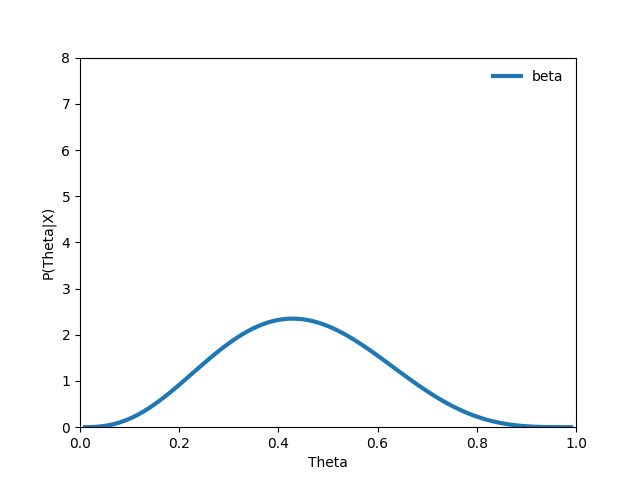
\includegraphics[width=0.45\textwidth, height=4cm]{2_by_5} }}
    \qquad
    \subfloat[\centering 20 heads out of 50]{{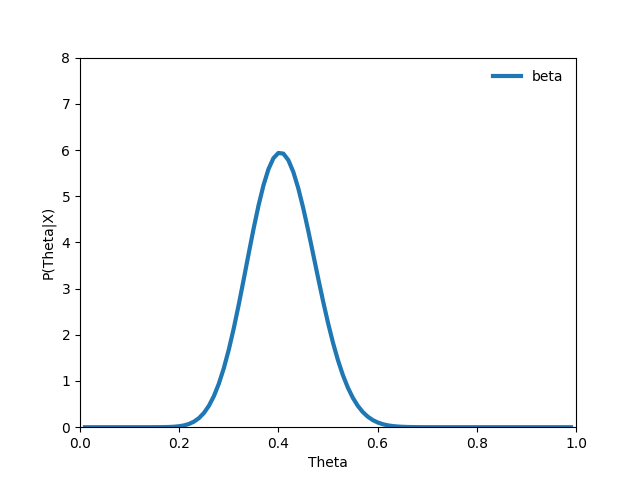
\includegraphics[width=0.45\textwidth, height=4cm]{20_by_50} }}\\
\caption{PDF of $P(\theta | X)$}
\end{figure}
\end{document}